
% --------------------------------------------------------------------
% This is a simple Beamer document that uses beamerthemesigma.sty
% Reading the comments should help you create a presentation even if
% you've never used Beamer before.
% --------------------------------------------------------------------
% Set our document class to Beamer
\documentclass[aspectratio=169]{beamer}

% Some packages for nice font encodings in the final PDF
\usepackage[utf8]{inputenc}
\usepackage[T1]{fontenc}

% From Jeff E
\usepackage{algo}

\usepackage{sigmastyle}

% To insert images
\usepackage{graphicx}

% Useful packages from the AMS
\usepackage{amsmath,amssymb,amsthm}

% Package for code highlighting
\usepackage{minted}
\setminted{breaklines=true, breakanywhere=true, style=default}

% Custom stuff for coins for first section
\usepackage{wasysym}
\usepackage{tikz}
\newcommand*\circled[1]{\tikz[baseline=(char.base)]{
            \node[shape=circle,draw,inner sep=2pt] (char) {#1};}}
\newcommand{\CP}{\circled{1}}
\newcommand{\CN}{\circled{5}}
\newcommand{\CD}{\circled{10}}
\newcommand{\CQ}{\circled{25}}
\newcommand{\CH}{\circled{50}}


% Set a title
\title{Generating Functions}

% The subtitle is generally where I'd expect you to put the week
% number, thus:
\subtitle{Week 11}
% \texorpdfstring to remove compilation warnings if you have math here

% Whoever worked on the presentation:
\author{Husnain}

% A date, if you'd like.
\date{}

% An institute name, if you're so inclined
% \institute{University of Illinois Urbana-Champaign}

% Use the SIGma theme for this Beamer presentation
\usetheme{sigma}
% --------------------------------------------------------------------
% Begin document
\begin{document}


% This frame is just the title.
\begin{frame}
\titlepage
\end{frame}

\section{Solving DP Problems quickly for Fun and Profit}
\frame{\sectionpage}

\begin{frame}
How many ways are there to make change for $N\cent$ with these coins? 

\vspace{10pt}

$$\circled{1},\; \circled{5},\; \circled{10},\; \circled{25},\; \circled{50}$$
\end{frame}

\begin{frame}
For example, we have that $16\cent$ can be represented in 6 different ways:
\begin{align*}
    16\cent &= \circled{10} \; \circled{5} \; \circled{1} \\
    &= \circled{5} \; \circled{5} \; \circled{5} \; \circled{1} \\
    &= \circled{10} \; \circled{1} \; \circled{1} \; \circled{1} \; \circled{1} \; \circled{1} \; \circled{1} \\
    &= \circled{5} \; \circled{5} \; \circled{1} \; \circled{1} \; \circled{1} \; \circled{1} \; \circled{1} \; \circled{1} \\
    &= \circled{5} \; \underbrace{\circled{1}\cdots\circled{1}}_{11} \\
    &= \underbrace{\circled{1}\cdots\circled{1}}_{16}
\end{align*}
\end{frame}

\begin{frame}[fragile]
\setminted{bgcolor=bg}
    \begin{minted}{python}
    @cache
    def num_coin_sums(N, coins):
        if N < 0: return 0
        if N == 0: return 1
        if len(coins) == 0: return 0
        return num_coin_sums(N - coins[0], coins) + num_coin_sums(N, tuple(coins[1:]))

    \end{minted}
\end{frame}

\begin{frame}
Consider a simpler problem - how many ways of making change with just dimes and nickels

\vspace{25pt}

To compact notation, let us denote $ \circled{1}^4 = \circled{1} \; \circled{1} \; \circled{1} \; \circled{1}$
\end{frame}

\begin{frame}

Consider all possible combinations of making change with  $\circled{5}$ and $\circled{10}$

\begin{align*}
5\cent &: \CN \\
10\cent &: \CD, \CN^2 \\
15\cent &: \CD \; \CN, \CN^3 \\
20\cent &: \CD^2, \CD \; \CN^2, \CN^4 \\
\vdots
\end{align*}

\end{frame}

\begin{frame}{WARNING: Engineering levels of rigor ahead\footnote{We will resolve this later}}

Consider the following sum of all combinations of nickels and dimes:

$$ S = 1 + \CN^0 + \CN + \CD + \CN^2 +  \CD \; \CN + \CN^3 +  \CD^2 + \CD \; \CN^2 + \CN^4  + \cdots $$

\end{frame}

\begin{frame}

\begin{align*}
S &= 1 + \CN + \CN^2 + \CN^3 + \CN^4 + \CN^5 + \cdots \\
&+ \CD + \CD \; \CN + \CD \; \CN^2 + \CD \; \CN^3 + \CD \; \CN^4 + \CD \; \CN^5 + \cdots \\
&+ \CD^2 + \CD^2 \; \CN + \CD^2 \; \CN^2 + \CD^2 \; \CN^3 + \CD^2 \; \CN^4 + \CD^2 \; \CN^5 + \cdots\\
&+ \CD^3  + \CD^3 \; \CN + \CD^3 \; \CN^2 + \CD^3 \; \CN^3 + \CD^3 \; \CN^4 + \CD^3 \; \CN^5 + \cdots \\
&+ \CD^4 + \CD^4 \; \CN + \CD^4 \; \CN^2 + \CD^4 \; \CN^3 + \CD^4 \; \CN^4 + \CD^4 \; \CN^5 \cdots \\
\vdots 
\end{align*}

\end{frame}

\begin{frame}
\begin{align*}
S &= 1 \left(1 + \CN + \CN^2 + \CN^3 + \CN^4 + \CN^5 + \cdots\right) \\
&+ \CD \left(1 + \CN + \CN^2 + \CN^3 + \CN^4 + \CN^5 + \cdots\right) \\
&+ \CD^2 \left(1 + \CN + \CN^2 + \CN^3 + \CN^4 + \CN^5 + \cdots\right) \cdots\\
&+ \CD^3  \left(1 + \CN + \CN^2 + \CN^3 + \CN^4 + \CN^5 + \cdots\right)  \cdots \\
&+ \CD^4 \left(1 + \CN + \CN^2 + \CN^3 + \CN^4 + \CN^5 + \cdots\right) \cdots \\
\vdots 
\end{align*}

\end{frame}

\begin{frame}
\begin{align*}
    \onslide<+->{S &= \left(1 + \CN + \CN^2 + \CN^3 + \cdots\right) \left(1 + \CD + \CD^2 + \CD^3 + \cdots\right)  \\}
        \onslide<+->{&= \frac{1}{1-\CN} \cdot \frac{1}{1-\CD} \hspace{1 in} \text{(geometric series)} \\}
        \onslide<+->{&= \frac{1}{1-x^5} \cdot \frac{1}{1-x^{10}} \hspace{1 in} \left(\CN = x^5, \CD = x^{10}\right)}
\end{align*}
\end{frame}

\begin{frame}[fragile]{Sanity Check}

We can check that this power series actually works

\begin{minted}{python}
    sage: R.<x> = PowerSeriesRing(ZZ, default_prec=100)
    sage: 1 / ((1-x^5) * (1-x^10))
    1 + x^5 + 2*x^10 + 2*x^15 + 3*x^20 + 3*x^25 + 4*x^30 + 4*x^35 + 5*x^40 + 5*x^45 + 6*x^50 + 6*x^55 + 7*x^60 + 7*x^65 + 8*x^70 + 8*x^75 + 9*x^80 + 9*x^85 + 10*x^90 + 10*x^95 + O(x^100)

\end{minted}

For example, there are only 8 ways to make $70\cent$ with nickles and dimes

\textbf{EXERCISE}: Check this

\end{frame}

\begin{frame}
By a similar kind of logic, letting $C_n$ being the number of ways of making change for $n \cent$, we have a \textbf{generating function}:

$$C(z) = \pause \sum_{n \ge 0} C_n z^n = \pause \frac{1}{(1-z)(1-z^5)(1-z^{10})(1-z^{25})(1-z^{50})}$$

\end{frame}

\begin{frame}[fragile]
With some algebraic manipulation of this generating function\footnote{See Knuth's \textit{Concrete Mathematics} p345-6 where this example is taken for the details of the derivation - it's mostly (messy) algebra}, we can get an explicit formula for its coefficients

    \begin{minted}{python}

from math import comb as C

def num_coin_sums_fast(N):
    A = [1,2,4,6,9,13,18,24,31,39,45,52,57,63,67,69,69,67,63,57,52,45,39,31,24,18,13,9,6,4,2,1]
    N //= 5
    q = N // 10; r = N % 10
    return A[r] * C(q+4, 4) + A[r+10] * C(q+3,4) + A[r+20] * C(q+2, 4) + A[r+30] * C(q+1, 4)

    \end{minted}


\end{frame}

%TODO: include benchmarks

\section{Ordinary Generating Functions}
\frame{\sectionpage}

\begin{frame}
We now define things more rigorously - define a \textbf{combinatorial class} to be a set of objects with a corresponding \textbf{size function}

\vspace{25pt}

In our previous example, our combinatorial class was $$ \mathcal{C} = \left\{ \CH^{z_1} \CQ^{z_2} \CD^{z_3} \CN^{z_4} \CP^{z_5} : z_i \in \mathbb{Z}_{\ge0} \right\}  $$

\vspace{25pt}

and the associated size function is $$ \left\|\CH^{z_1} \CQ^{z_2} \CD^{z_3} \CN^{z_4} \CP^{z_5} \right\| = 50z_1 + 25z_2 + 10z_3 + 5z_4 + z_5 $$


\end{frame}

\begin{frame}

For any combinatorial class $A$, we define it's associated \textbf{ordinary generating function} to be

$$ A(z) = \sum_{ a \in A } z^{|a|} = \sum_{N \ge 0} A_N z^N $$ 

\pause
\vspace{25pt}


With this generating function, we can get the number of objects of size $N$ by \textbf{extracting the corresponding coefficient}

$$ A_N = [z^N] A(z) $$

\end{frame}

\begin{frame}

In our last example, we had  $ C(z) = \frac{1}{(1-z)(1-z^5)(1-z^{10})(1-z^{25})(1-z^{50})}$ 

We can use this to count the number of ways of getting $42 \cent$ as follows:

\begin{align*}
C_{42} &= [z^{42}] C(z) \\
&= [z^{42}] \left( 1 + z + z^2 + z^3 + z^4 + 2z^5 + \cdots + 31 z^{41} + \underline{31 z^{42}} + \cdots \right) \\
&= 31
\end{align*}

\end{frame}

\begin{frame}{Exercises}

We will be working over binary strings - assume the size function is just the length of the string

Find the corresponding generating function for these combiatorial classes
\begin{itemize}
    \item  $\Sigma$ = all binary strings
    \item  $\mathcal{Z}$ = the set of all strings of zeros of length at least 5
    \item  $\mathcal{E}$ = the set of all binary strings whose length is even
\end{itemize}

\end{frame}

\begin{frame}
$$ \Sigma(z) = \sum_{N \ge 0} 2^N z^N = \sum_{N \ge 0} (2z)^N = \frac{1}{1-2z} $$
$$ \mathcal{Z}(z) = \sum_{N \ge 5} z^N = \frac{z^5}{1-z}  $$
$$ \mathcal{E}(z) = \sum_{N \ge 0} 2^{2N} z^{2N} = \frac{1}{1-4z^2} $$
\end{frame}

\begin{frame}

Let $\mathcal{A}$ and $\mathcal{B}$ be combinatorial classes with associated generating functions $A(z)$ and $B(z)$ respectively. 
\vspace{25pt}

We can combine these combinatorial classes to get new combinatorial classes with new generating functions

\end{frame}

\begin{frame}

Let $ \mathcal{C} = \mathcal{A} + \mathcal{B} $ be the disjoint union of $\mathcal{A}$ and $\mathcal{B} $. We have that the corresponding generating function is 

$$ C(z) = \pause \sum_{c \in \mathcal{A} + \mathcal{B}} z^{|c|} = \pause \sum_{a \in \mathcal{A}} z^{|a|} + \sum_{b \in \mathcal{B}} z^{|b|} = \pause A(z) + B(z) $$

\end{frame}

\begin{frame}
Similarly, we have that if $ \mathcal{C} = \mathcal{A} \times \mathcal{B} $ be the Cartesian product of $\mathcal{A}$ and $\mathcal{B}$. then the corresponding generating function is

\vspace{25pt}

$$ C(z) = \pause \sum_{c \in \mathcal{A} \times \mathcal{B}} z^{|c|} = \pause \sum_{a \in \mathcal{A}} \sum_{b \in \mathcal{B}} z^{|a|+|b|}= \pause \left(  \sum_{a \in \mathcal{A}} z^{|a| }\right) \left( \sum_{b \in \mathcal{B}} z^{|b|}\right) = \pause A(z) B(z) \pause $$ 
\end{frame}

\begin{frame}
    Finally, letting $\epsilon$ be the empty combinatorial class, let $\mathcal{C} = \epsilon + A + A^2 + A^3 + ... \equiv \text{SEQ}(A) $, we have that the corresponding generating function is $C(z) = \frac{1}{1-A(z)}$
\end{frame}

\begin{frame}

With these new tools, we can solve the above problems much more easily.

\vspace{25pt}

For example:

$$ B = \{ \texttt{0}, \texttt{1} \}, B(z) = 2z \implies \Sigma = \text{SEQ}(B), \Sigma(z) = \frac{1}{1-2z} $$

\end{frame}

\section*{A Harder Example}

\begin{frame}

Let's deal with something more complicated: how many binary trees are there with $n$ internal nodes (and therefore $n+1$ leaf nodes)?

An example for $ n = 3 $:

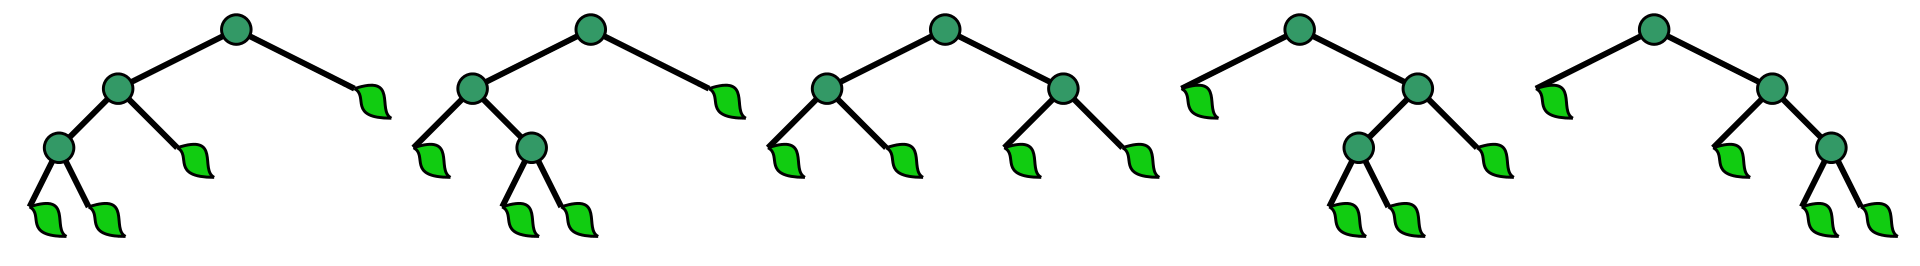
\includegraphics[width=\textwidth]{trees.png}

\end{frame}
Let $\mathcal{T}$ be the combinatorial class of all such trees. Note that we can decompose any tree $T$ as follows:

\begin{center}
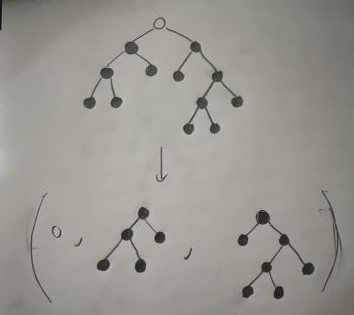
\includegraphics[width=0.6\textwidth]{tree_decomp.jpg}
\end{center}

\begin{frame}
Note that we have an invertible mapping $ T \mapsto (\circ, T_l, T_r) $ meaning that we can decompose and recompose tress uniquely.

\vspace{25pt}

Since the left and right subtrees are also in $\mathcal{T}$, we can use the above to come up with an equation defining $\mathcal{T}$ and get a generating function $T(z)$:

$$ \mathcal{T} = \circ + \mathcal{T} \times \mathcal{T} \implies T(z) = z + T(z)^2 \implies T(z) = \frac{1 - \sqrt{1-4z}}{2} $$ 

\end{frame}

\begin{frame}
    With this generating function, we can get a general formula for the $n^{th}$ coefficient $T_n$ (Note that this is generally not possible) \pause
    \begin{align*}
        \onslide<+->{(1 - 4z)^{1/2} &= \sum_{k \ge 0} \binom{\frac{1}{2}}{k} (-4z)^k \\}
        \onslide<+->{\implies T(z) &= \frac{1 - \sqrt{1-4z}}{2} = -\frac{1}{2} \sum_{k \ge 1} \binom{\frac{1}{2}}{k} (-4z)^k \\}
        \onslide<+->{\implies T_n &= -\frac{1}{2} \binom{\frac{1}{2}}{k} (-4)^k = \frac{1}{n} \binom{2n-2}{n-1}}
    \end{align*}

\end{frame}

\begin{frame}

These are the \textbf{Catalan numbers} - Richard Stanley has \href{https://www.cambridge.org/core/books/catalan-numbers/5441FB5B09E9C01185834D9CBB9DFAD9}{207 examples} of different sequences that correspond to the Catalan numbers

\end{frame}

\begin{frame}
We conclude from an example from number theory - let $p_n$ be the number of \textbf{partitions} of $n$, or the number of ways of writing $n$ as a sum of positive integers.

\vspace{25pt}

\pause
For example, we have $p_5 = 7$ as 

\begin{align*}
5 &= 5 \\
&= 4+1 \\
&= 3+2 \\
&= 3+1+1 \\
&= 2+2+1 \\
&= 2+1+1+1 \\
&= 1+1+1+1+1
\end{align*}
\end{frame}

\begin{frame}
Similar to our first example, we can define a generating function $ P(z) = \sum_{k \ge 0} p_k z^k $

\begin{align*}
P(z) &= \sum_{k \ge 0} p_k z^k \\
&= (1 + z^1 + z^{1+1} + \cdots)(1 + z^2 + z^{2+2} + \cdots)(1 + z^{3}+ z^{3+3} + \cdots) \cdots \\
&= \prod_{j \ge 1} \frac{1}{1-x^j}
\end{align*}

\end{frame}

\begin{frame}

We end with a proof of a non-obvious fact


Let $ P_o(n) $ be the number of partitions of $n$ into \textit{odd} parts. For example, we have that $ P_o(7) = 5 $ as

\begin{align*}
7 &= 7 \\
&= 5 + 1 + 1 \\
&= 3 + 3 + 1 \\
&= 3 + 1 + 1 + 1 + 1 \\
&= 1 + 1 + 1 + 1 + 1 + 1 + 1
\end{align*}

\end{frame}

\begin{frame}

Next, let $P_d(n)$ be the number of partitions of $n$ into \textit{distinct} parts. For example, we have that $ P_d(7) = 5$ as

\begin{align*}
7 &= 7 \\
&= 6 + 1\\
&= 5 + 2 \\
&= 4 + 3\\
&= 4 + 2 + 1
\end{align*}

\end{frame}


\begin{frame}

This equality is not a coincidence - we will show that $ P_o(n) = P_d(n)$ for any $n$.

Let $$P_o(z) = \sum_{k \ge 0} P_o(k) z^k \;\; , \;\; P_d(z) = \sum_{k \ge 0} P_d(k) z^k $$ be the corresponding generating functions.

\end{frame}

\begin{frame}{The Proof}
We have:
\begin{align*}
P_d(z) =~& (1 + z)(1 + z^2)(1 + z^3)(1 + z^4)(1 + z^5)\cdots \\
\onslide<+->{=~&\dfrac{1 - z^2}{1 - z} \cdot \dfrac{1 - z^4}{1 - z^2} \cdot \dfrac{1 - z^6}{1 - z^3} \cdot \dfrac{1 - z^8}{1 - z^4} \cdot \dfrac{1 - z^{10}}{1 - z^5} \cdots \\}
\onslide<+->{=~& \dfrac{1}{(1 - z)(1-z^3)(1-z^5) \cdots} \\}
\onslide<+->{=~& (1 + z^{1} + z^{1+1} + z^{1+1+1} + \cdots) (1 + z^{3} + z^{3+3} + z^{3+3+3} + \cdots)\\ &(1 + z^{5} + z^{5+5} + z^{5+5+5} + \cdots) \cdots \\}
\onslide<+->{=~& P_o(z)}
\end{align*}\pause

Since these two sequences have the same generating function, their coefficients must be the same - ending the proof. 
\end{frame}

\begin{frame}{Further Resources}
\begin{itemize}
 \item \href{https://www2.math.upenn.edu/~wilf/gfologyLinked2.pdf}{\textit{generatingfunctionology} by Herbert Wilf} - good overall resource on generating functions
 \item \href{http://algo.inria.fr/flajolet/Publications/book.pdf}{\textit{Analytic Combinatorics} by Sedgewick and Flajolet} - longer resource on generating functions that details the symbolic method (detailed in the presentation) and how to deal with generating functions using complex analysis to get asymptotic information
 \item \href{https://www.csie.ntu.edu.tw/~r97002/temp/Concrete\%20Mathematics\%202e.pdf}{\textit{Concrete Mathematics} by Graham, Knuth and Patashnik} - the Bible on any mathematics you may need for computer science; has a chapter on generating functions that was referenced
\end{itemize}

\end{frame}


\font\eightss=cmssq8
\font\eightssi=cmssqi8
\newcommand\quoteAuthorDate[3]{\begingroup
  \baselineskip 10pt
  \parfillskip 0pt
  \interlinepenalty 10000 % not needed in example
  \leftskip 0pt plus 40pc minus \parindent
  \let\rm=\eightss
  \let\sl=\eightssi
  \everypar{\sl}#1\par
  \nobreak\smallskip
  \noindent\rm--- #2\unskip\enspace(#3)\par
  \endgroup}
\begin{frame}
    \begin{center}
        \item \quoteAuthorDate{A generating function is a clothesline on which we hang up a sequence of numbers for display.}{HERBERT WILF}{1990}
    \end{center}
\end{frame}

\end{document}
